\chapter{Can Fear End?}

This chapter follows J. Krishnamurti's San Diego 1970 public talk on whether the human mind can be completely free of fear, source material preserved by the Krishnamurti Foundation Trust and curated for this course by LazyingArt LLC through Video2Book. There are no validated blackboard frames or equations for this lecture, so the mathematical structure below is deliberately schematic: it is a disciplined notation for the movement of the inquiry, not an imported psychology or a formal theory. We use arrows only as reading aids, to keep the sequence of the spoken investigation visible on the page.

\section{Seriousness, Joy, And The Refusal To Accept Fear}

Krishnamurti begins with a claim about seriousness. Seriousness is not grimness, and it does not exclude joy or enjoyment. But as long as there is fear, he says, one cannot be serious in the full sense, and one cannot know what great joy means. Fear is not introduced as one emotion among others; it is introduced as a condition that distorts the whole field of living.

The first move, then, is not to define fear but to see why the inquiry has urgency. We have accepted fear, just as we have accepted violence, as a way of life. We have grown used to being physically and psychologically afraid. The lecture asks whether this acceptance can end, not gradually in theory, but in the act of attending.

A compact way to mark the opening relation is

\begin{equation}
\text{fear present}
\quad \Longrightarrow \quad
\text{seriousness, enjoyment, and joy are obstructed}.
\end{equation}

This is not a causal law in the scientific sense. It is the starting constraint of the inquiry. If the mind is afraid, its action, pleasure, relationship, and thought are already moving under pressure.

\section{Communication As Shared Inquiry}

Before the lecture can examine fear, it asks how we are going to listen. Communication, in Krishnamurti's use here, is not transmission from the speaker to a passive audience. It means creating together, understanding together, and working together. The listener is not asked to accept, deny, agree, disagree, or compare what is being said with accumulated knowledge.

This matters because fear cannot be looked at through a mind already occupied with conclusions. If we are interpreting, translating, judging, or measuring while listening, then the very instrument of inquiry is not clear. Krishnamurti gives the image of a microscope: if the instrument is dull, the seeing is distorted.

We may record the condition of inquiry as follows:

\begin{align}
\text{attention} &\neq \text{agreement},\\
\text{attention} &\neq \text{disagreement},\\
\text{attention} &\neq \text{comparison with what is already known}.
\end{align}

The point is simple but strict. We are not building a doctrine about fear. We are attempting to observe fear with an instrument that is not already clouded by prejudice, conclusion, or resistance.

\section{From Many Fears To The Structure Of Fear}

The lecture next opens out the range of fear. There is fear of the dark, fear of wife or husband, fear of public opinion, fear of loneliness, fear of emptiness, fear of the future, fear of insecurity, fear of death, fear of failure, fear of not being somebody. There are conscious fears and hidden fears. There is fear of time: fear of what happened yesterday, fear that pain will return tomorrow, fear of growing old, depending on another, becoming senile.

Krishnamurti does not propose to examine each fear separately. That would take an enormous amount of time, and it would never reach the structure. The lecture therefore pivots from the inventory of fears to their common movement. Fear is described as a movement away from what is.

\begin{equation}
\text{fear}
\;\sim\;
\text{movement away from what is}.
\end{equation}

The symbol \(\sim\) is only a note-taking sign. It says that in this lecture fear is to be watched as a movement: flight, escape, avoidance, comparison, and the search for something other than the actual fact.

Comparison is one of the clearest instances of that movement. The mind compares itself with another, or compares what it is with what it thinks it should be. In that comparison there is distance, and in that distance fear is bred.

\begin{equation}
\text{comparison}
\;\longrightarrow\;
\text{distance from what is}
\;\longrightarrow\;
\text{fear}.
\end{equation}

The important distinction is that fear is not primarily the object to which one escapes. It is the movement of escape itself. This distinction will govern the rest of the chapter.

\begin{figure}
\centering
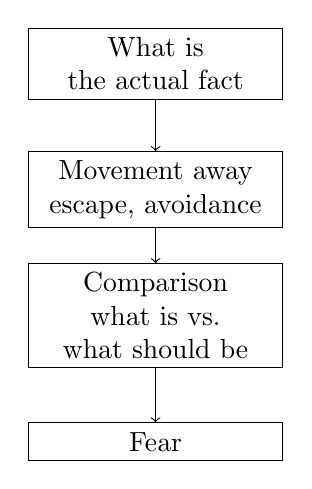
\begin{tikzpicture}
\node[draw, text width=3.0cm, align=center] (a) at (0,0) {What is\\the actual fact};
\node[draw, text width=3.0cm, align=center] (b) at (0,-1.6) {Movement away\\escape, avoidance};
\node[draw, text width=3.0cm, align=center] (c) at (0,-3.2) {Comparison\\what is vs. what should be};
\node[draw, text width=3.0cm, align=center] (d) at (0,-4.8) {Fear};
\draw[->] (a) -- (b);
\draw[->] (b) -- (c);
\draw[->] (c) -- (d);
\end{tikzpicture}
\caption{A transcript-based reconstruction of the lecture's first structural claim: fear is approached as movement away from what is.}
\end{figure}

\section{Will, Analysis, And Dreams}

Once fear is understood as movement away from what is, the familiar solutions become suspect. Will appears first. The mind says, ``I will not be afraid.'' But this is still a movement against fear. It does not understand fear; it opposes it. For that reason Krishnamurti says that the act of will has no meaning here.

\subsection{Question \& Answer}

\paragraph{Question.} If there are conscious fears and also hidden fears, how are those hidden fears to be exposed? Can they be exposed through analysis, and can analysis free the mind from fear?

\paragraph{Answer.} Krishnamurti's answer is no. Analysis implies time. It also implies an analyser. The analyser is not outside the field of fear; it is a fragment among the many fragments that make up the ``me,'' the ``I,'' the ego. The analyser then assumes authority and tries to analyse the fear which it has itself helped to create.

The structure of analysis may be written schematically:

\begin{equation}
\text{analysis}
\;\longrightarrow\;
\text{time} + \text{analyser} + \text{division}.
\end{equation}

And the lecture's conclusion is

\begin{equation}
\text{analysis}
\;\not\longrightarrow\;
\text{ending of fear}.
\end{equation}

The reason is not merely that analysis is slow. The deeper reason is that analysis divides. It sets up an analyser separate from the thing analysed. That division belongs to the very structure of the ``me'' that is already implicated in fear.

\begin{proof}
The argument in the lecture can be laid out step by step.
\begin{enumerate}
\item Hidden fear seems to require exposure.
\item Analysis proposes to expose fear by examining causes.
\item Analysis takes time, perhaps years or a whole life.
\item Analysis also requires an analyser.
\item The analyser is not independent of conditioning; it is a fragment of the ``me.''
\item The analyser separates itself from fear and treats fear as an object.
\item That separation is division.
\item Division sustains conflict and does not end fear.
\end{enumerate}
Therefore, in this inquiry, analysis cannot be the way to the ending of fear.
\end{proof}

The lecture then asks whether dreams provide another route. Perhaps hidden fears are exposed in dreams. But Krishnamurti rejects this as well. Dreams are described as the continuation of waking movement: doing, acting, and something happening, just as in waking hours. Dreams therefore do not stand outside the movement; they continue it.

\begin{table}
\centering
\begin{tabular}{p{0.25\linewidth} p{0.55\linewidth}}
Route & Why it fails in this inquiry \\
Will & It is a movement against fear, not understanding fear. \\
Analysis & It implies time, an analyser, and division. \\
Dreams & They continue the movement of waking hours. \\
Progressive change & It postpones ending and keeps fear within time. \\
\end{tabular}
\caption{Rejected routes, stated only in the terms used by the lecture.}
\end{table}

After these eliminations, the mind is not being deprived of tools for the sake of negation. It is being made sensitive. The accustomed routes are set aside so that fear can be looked at directly.

\section{Thought, Memory, Pleasure, And Fear}

The next movement of the lecture begins with a renewed question: what is fear, and how does it come? Fear is always in relation to something. It does not exist by itself. There is fear of what happened yesterday and fear that it may happen again tomorrow. There is a fixed point, a remembered event, from which relationship takes place.

A simple example carries the argument. There was pain yesterday. There is memory of that pain. Thought returns to the memory and projects its repetition tomorrow. That projection is fear.

\begin{align}
\text{past pain}
&\longrightarrow \text{memory} \\
&\longrightarrow \text{thought of repetition} \\
&\longrightarrow \text{fear of tomorrow}.
\end{align}

This is the chapter's clearest worked example. We can spell it out.

\paragraph{Example.} Suppose there was pain yesterday. If there were only the fact that pain occurred, the matter would end there. But memory retains the pain. Thought then says, in effect, ``It may happen again.'' The remembered past is projected as a possible future. The mind is no longer with the simple fact of past pain; it is living in the image of repetition. In that projection, fear has entered.

This is why the lecture says that thought brings about fear. But Krishnamurti immediately adds that thought also cultivates pleasure. To understand fear, one must understand pleasure, because they are interrelated. One cannot demand only pleasure and no fear, since fear is the other side of the coin called pleasure.

The parallel structure is:

\begin{align}
\text{past pleasure}
&\longrightarrow \text{image or thought} \\
&\longrightarrow \text{desire for repetition} \\
&\longrightarrow \text{fear of loss or frustration}.
\end{align}

The same operation appears in both chains. Thought remembers, forms an image, and projects into tomorrow. In the case of pain, projection becomes fear of repetition. In the case of pleasure, projection becomes desire for repetition and fear that the pleasure may not return.

\begin{figure}
\centering
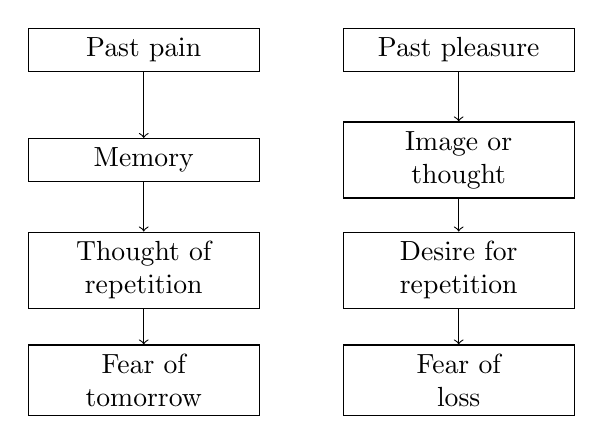
\begin{tikzpicture}
\node[draw, text width=2.7cm, align=center] (p1) at (-2.0,0) {Past pain};
\node[draw, text width=2.7cm, align=center] (p2) at (-2.0,-1.4) {Memory};
\node[draw, text width=2.7cm, align=center] (p3) at (-2.0,-2.8) {Thought of\\repetition};
\node[draw, text width=2.7cm, align=center] (p4) at (-2.0,-4.2) {Fear of\\tomorrow};

\node[draw, text width=2.7cm, align=center] (q1) at (2.0,0) {Past pleasure};
\node[draw, text width=2.7cm, align=center] (q2) at (2.0,-1.4) {Image or\\thought};
\node[draw, text width=2.7cm, align=center] (q3) at (2.0,-2.8) {Desire for\\repetition};
\node[draw, text width=2.7cm, align=center] (q4) at (2.0,-4.2) {Fear of\\loss};

\draw[->] (p1) -- (p2);
\draw[->] (p2) -- (p3);
\draw[->] (p3) -- (p4);

\draw[->] (q1) -- (q2);
\draw[->] (q2) -- (q3);
\draw[->] (q3) -- (q4);
\end{tikzpicture}
\caption{Two transcript-based chains showing how thought sustains both fear and pleasure.}
\end{figure}

Joy is then carefully distinguished from pleasure. Pleasure can be cultivated by thought, repeated in image, pursued, and remembered. Joy cannot. The moment thought tries to cultivate joy, it becomes a remembered pleasure, and therefore something one is afraid to lose.

Thus the relation is not

\begin{equation}
\text{joy} = \text{pleasure}.
\end{equation}

Rather, in the lecture's distinction,

\begin{equation}
\text{pleasure is sustained by thought},
\qquad
\text{joy is not the product of thought}.
\end{equation}

This distinction matters for the whole book's inquiry into happiness. Pleasure, fear, and thought form a circuit; joy does not belong to that circuit.

\section{What Is The Mind To Do With Thought?}

At this point the lecture reaches its central difficulty. If thought is doing all this, what is one to do? Thought has brought in time as a means of escaping fear while sustaining fear. Thought nourishes pleasure. Thought separates itself as the analyser. Thought is responsible for pleasure, pain, and fear.

But thought cannot simply be killed, destroyed, forgotten, or resisted. If one resists thought, that resistance is another form of thought. More importantly, thought is necessary. Memory is needed to function daily: to speak, to go home, to work, to use technical knowledge, to earn a livelihood.

We therefore have a two-sided fact:

\begin{align}
\text{thought} &\longrightarrow \text{practical function},\\
\text{thought} &\longrightarrow \text{psychological fear}.
\end{align}

This is not a contradiction to be solved by suppressing thought. It is a fact to be seen with precision.

\subsection{Question \& Answer}

\paragraph{Question.} If thought must function efficiently and sanely in daily life, and yet that very thought breeds fear, what is the mind to do?

\paragraph{Answer.} Krishnamurti does not answer by giving a method. Before answering, he asks what is the state of the mind that has gone through the inquiry. Has it actually seen the facts of analysis, time, escape, dependency, comparison, pleasure, and fear? If it has, then the mind has become sensitive, intelligent, and alive by throwing off accumulated burdens. Only such a mind can look at the question without turning the answer into another formula.

This pause is essential. The answer depends on the quality of observation, not on a technique. If the inquiry has been merely verbal, then the mind has no real answer. If the inquiry has been lived step by step while listening, then the mind can look at the whole process of thinking.

\section{The Centre, Naming, And Division}

The final movement asks whether there is a centre from which one thinks. The centre is the censor, the one who judges, evaluates, condemns, and justifies. Krishnamurti identifies it as the ``me'': my opinions, my country, my experience, my possessions, my relationships, my beliefs. From that centre we act and think.

The centre divides. Because it divides, there is conflict. If the mind observes fear from that centre, it is still caught in fear. The centre has separated itself from the thing it calls fear and then says, ``I must get rid of it,'' ``I must analyse it,'' ``I must overcome it,'' ``I must resist it.'' In that movement it strengthens fear.

We may represent the movement as follows:

\begin{equation}
\text{centre/me}
\longrightarrow
\text{division}
\longrightarrow
\text{conflict and resistance}
\longrightarrow
\text{fear strengthened}.
\end{equation}

Naming is part of the same operation. The moment the mind says ``fear,'' it has named the fact. Naming brings in the past, because the name comes from memory. It also divides: the namer and the named, the observer and the observed, the centre and fear.

\begin{equation}
\text{naming}
\longrightarrow
\text{past} + \text{division}.
\end{equation}

So the closing question is exact: can the mind look at fear without the centre and without naming it? This is not a trick of language. It is the end of the movement that has sustained fear through division.

\begin{figure}
\centering
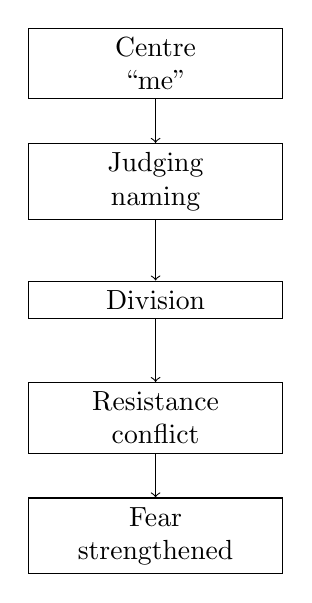
\begin{tikzpicture}
\node[draw, text width=3.0cm, align=center] (a) at (0,0) {Centre\\``me''};
\node[draw, text width=3.0cm, align=center] (b) at (0,-1.5) {Judging\\naming};
\node[draw, text width=3.0cm, align=center] (c) at (0,-3.0) {Division};
\node[draw, text width=3.0cm, align=center] (d) at (0,-4.5) {Resistance\\conflict};
\node[draw, text width=3.0cm, align=center] (e) at (0,-6.0) {Fear\\strengthened};
\draw[->] (a) -- (b);
\draw[->] (b) -- (c);
\draw[->] (c) -- (d);
\draw[->] (d) -- (e);
\end{tikzpicture}
\caption{The centre strengthens fear by dividing itself from what it calls fear.}
\end{figure}

The alternative is stated with care:

\begin{equation}
\text{observation without centre and without naming}
\longrightarrow
\text{ending of fear}.
\end{equation}

Here again the arrow is not a mechanical promise. It records the lecture's conclusion. When the mind observes closely, with care, affection, and attention, without the accustomed division of a centre, fear ends both in its hidden and open forms.

\section{Summary}

The lecture begins with the seriousness of fear and ends with direct observation. Its movement is not from problem to technique but from confusion to seeing. First, fear is shown to obstruct seriousness and joy. Then the inquiry establishes its own condition: communication without acceptance, denial, comparison, or conclusion. The many forms of fear are gathered into a structure: fear as movement away from what is.

The usual routes are then set aside. Will is another movement against fear. Analysis implies time, an analyser, and division. Dreams continue the waking movement. This clearing prepares the central insight: thought, through memory and projection, sustains both fear and pleasure. Yet thought is also necessary for ordinary life, so it cannot simply be destroyed.

The final distinction is the centre. The ``me'' divides itself from fear, names it, judges it, resists it, and thereby strengthens it. The lecture's answer is not a method of suppression but an observation without that centre and without naming. In that attention, Krishnamurti says, there is the ending of fear.